\documentclass[heading.tex]{subfiles}
\setcounter{secnumdepth}{4}
\setcounter{tocdepth}{4}
\begin{document}

\section{Introduction}

	Aerospace engineers have promoted tube transport over the course of a century;
	the most prominent include Robert Goddard \cite{Goddard} (creator of the first liquid fueld
	rocket) to Dr. Robert Salter (a forefather of the satellite). As early as 1972,
	a study conducted by the RAND coperation concluded that high-speed `tubecraft'
	was technologically feasible with political pressure being the greatest
	obstacle.\cite{RAND} National interest was once again rekindled in 2013 with a refreshed
	Hyperloop concept championed by Elon Musk, CEO of Space Exploration
	Technologies (SpaceX) and Tesla Motors.\cite{Musk}
	Unlike previous waves of interest, the currently
	popularized design has spurred widespread international development efforts
	amongst hundreds of leading universities, private companies with over \$100M
	in venture capitalist backing, and smaller research efforts at NASA and the
	US Department of Transportation. \cite{Chin}
	The design has continously evolved, with the latest Hyperloop derivative
	generating lift using magnetic levitation.
	In the same way an airplane is differentiated from an airship,
	or a hydroplane is differentiated from a boat,
	Magneplane is a plane in the sense that it generates lift dynamically
	by moving over a medium at high-speeds,
	rather than depending on buoyancy or static phenomena.
	It's transonic operation, air-breathing flow-path and aerodynamic
	driven design all qualify it as a plane over a train.
	The concept deviates from existing high-speed rail designs by eliminating
	the rails, enclosing the passenger pod in a tube under a partial vacuum,
	with propulsion handled by a set of linear electromagnetic accelerators
	mounted to the tube. The entire system is held either above ground on concrete
	columns or subterranian tunnels maintaining a relatively straight trajectory.

	\begin{figure}[hbtp]
		\centering
		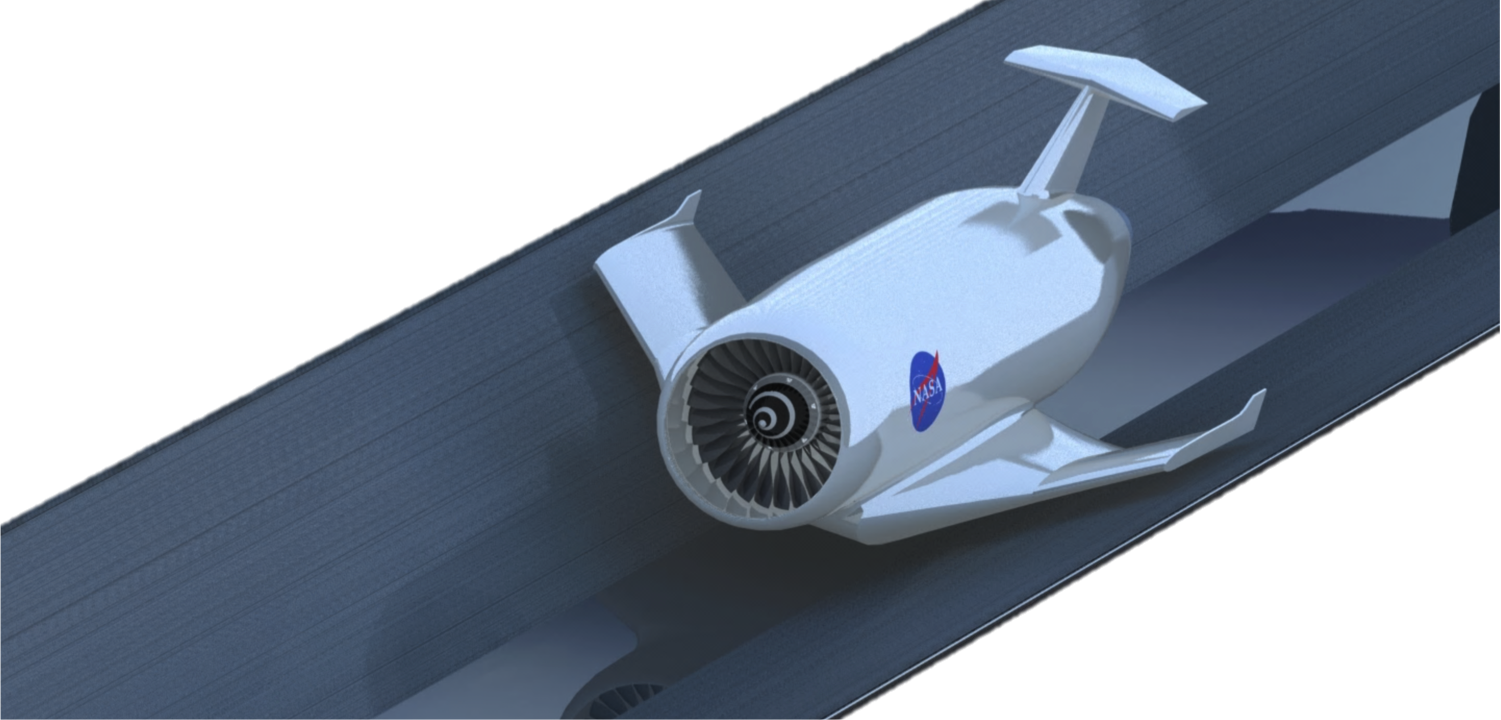
\includegraphics[width=.85\textwidth]{images/MagnePlane.png}
		\caption[MagnePlane Concept Sketch]{MagnePlane-alpha concept of the passenger pod.}
		\label{f:hyperloopSketch}
	\end{figure}

\section{Global Growth in Demand for High Speed Mobility}
	\label{s:demand}

	The MagnePlane vehicle flies low enough that propulsion can be offloaded to
	ground systems rivaling efficiencies previously limited to terrestrial
	vehicles. By sacrificing an airplane’s traditional mission flexibility,
	it’s optimized for passenger throughput, door-to-door travel time, and energy
	efficiency.
	The concept is best-suited for distances between 250-500 nautical miles,
	which comprised 57\% of commercial aircraft fleet operations in 2012.

	\begin{figure}[H]
		\centering
		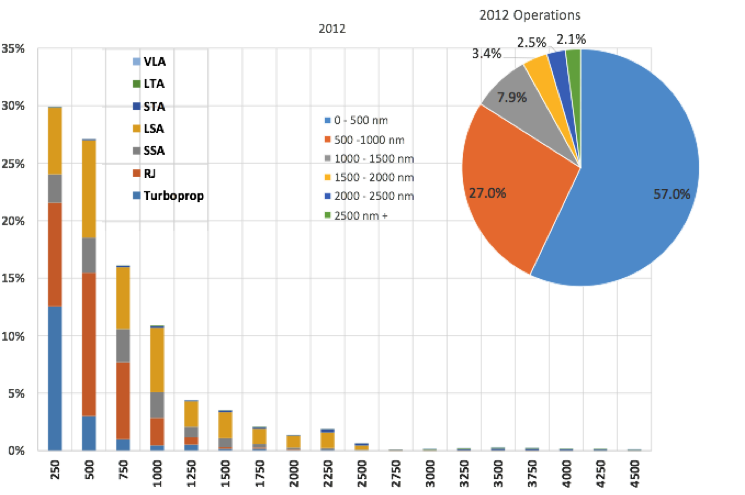
\includegraphics[width=.75\textwidth]{images/Pie.png}
		\caption[FleetOps]{Credit: AATT, Mark Guynn. The bar graph plots percentage of 2012 fleet operations versus mission distance, aircraft type is distinguished by color. Alternatively the pie chart breaks down operations into six groups based on distance alone.}
		\label{f:fleetOps}
	\end{figure}

	As stressed in NASA's Strategic Implementation Plan, operations must keep pace
	with both an overall growing transportation market and simultaneous growth in
	market share dedicated to high-speed transport. By 2050, 41\% of world traffic
	market share will be high-speed transport. \cite{Schafer}

	Hyperloop offers a compelling opportunity to offset this congestion. In terms of travel speed and door-to-door travel time, it's designed to occupy a highly desired gap between existing ground and air travel modes.

	\begin{figure}[hbtp]
		\centering
		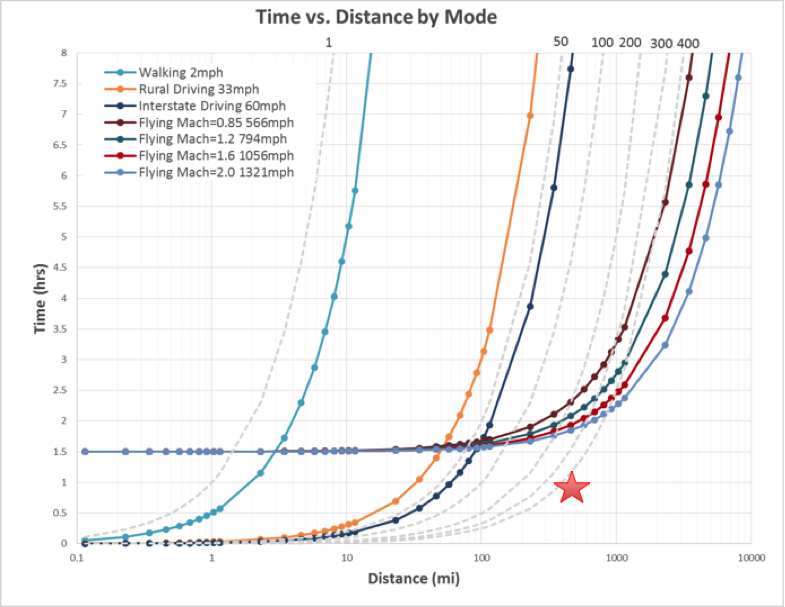
\includegraphics[width=.75\textwidth]{images/Seidel.png}
		\caption[Time]{Relationship between travel time and distance, across multiple travel modes. Hyperloop offers innovation in passenger boarding, and delays associated with runway taxi, holding patterns, and other issues exacerbated by airport congestion. Source: NASA CAS Big Questions Workshop, G. Welch, J. Seidel}
		\label{f:time}
	\end{figure}

	Furthermore, Hyperloop is positioned in the segment of the aeronautics market most sensitive to technology improvements. Optimizing operations in the 200-500 mile range is estimated to have the greatest effect on demand for person trips per year in 2025 as shown in Figure \ref{f:demand}.

	\begin{figure}[hbtp]
		\centering
		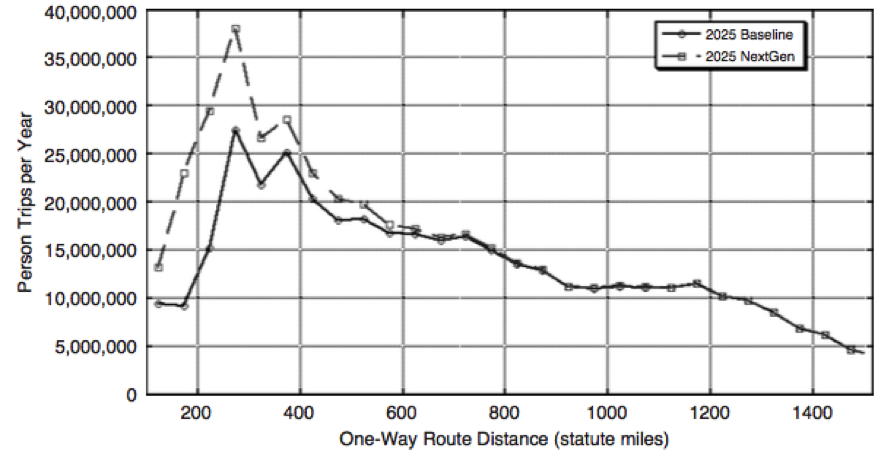
\includegraphics[width=.75\textwidth]{images/demand.png}
		\caption[demand]{Potential increase in commercial airline demand because of NextGen. Source: Forecasting Model for Air Taxi, Commercial Airline, and Automobile Demand in the United States, H. Baik, et al.}
		\label{f:demand}
	\end{figure}

	This critical range also coincides with the
	most price sensitive region of air travel.
	Beyond speed and energy efficiency,
	Hyperloop offers a unique high throughput
	capability relative to conventional aircraft.
	This departure from typical aircraft constraints
	is intended to provide a compelling price point
	at a time where automobile vehicle miles are
	projected to increase by 7 billion when airline
	fares increase by 10\% in 2015 as shown in Figure \ref{f:price}.

	\begin{figure}[hbtp]
		\centering
		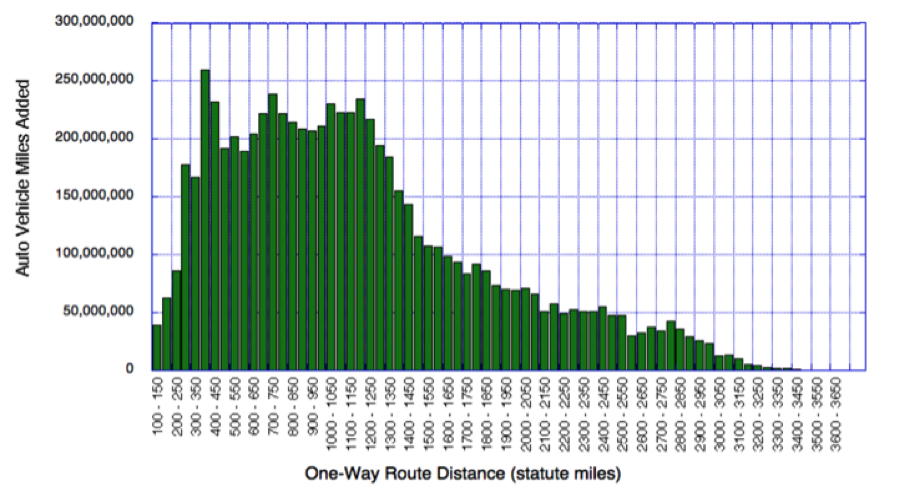
\includegraphics[width=.75\textwidth]{images/price.png}
		\caption[price]{Distribution of displaced aircraft miles due to a 10\% increase in ticket cost}
		\label{f:price}
	\end{figure}


\section{Hyperloop Model Overview}

	The model expands on previous works \cite{Chin} \textsuperscript{,}
	\cite{goodwin2009cantera}\textsuperscript{,} \cite{GrayBenchmarking2013}
	and is built using OpenMDAO, a python-based modeling and optimizaiton framework.
	This work focuses on thermodynamic, aerodnymanic, structural,
	weight, sensor and power considerations, with additional calculations for cost
	and mission design. The full system model integrates multiple discpline tools
	including Fun3D, Pointwise, AFLR3, SUPIN, NPSS, Solidworks, PyCycle, Pointer,
	and Engineering Sketch Pad. OpenMDAO is used for it's built in drivers, solvers,
	optimizers, database recorders, external-code wrappers as well as it's
	mathematical derivative management. Each discpline is further discussed in the
	following sections.

	\subfile{HyperloopModelOverview}

	\label{s:struct}

	\begin{figure}[hbtp]
		\centering
		\includegraphics[width=0.65\textwidth]{images/TopAssembly.png}
		\caption{Workflow and dependencies between the top-level Hyperloop assemblies.}
		\label{f:hyperloopXDSM}
	\end{figure}

\section{Compressor Power and Battery Sizing}

	\begin{figure}[hbtp]
		\centering
		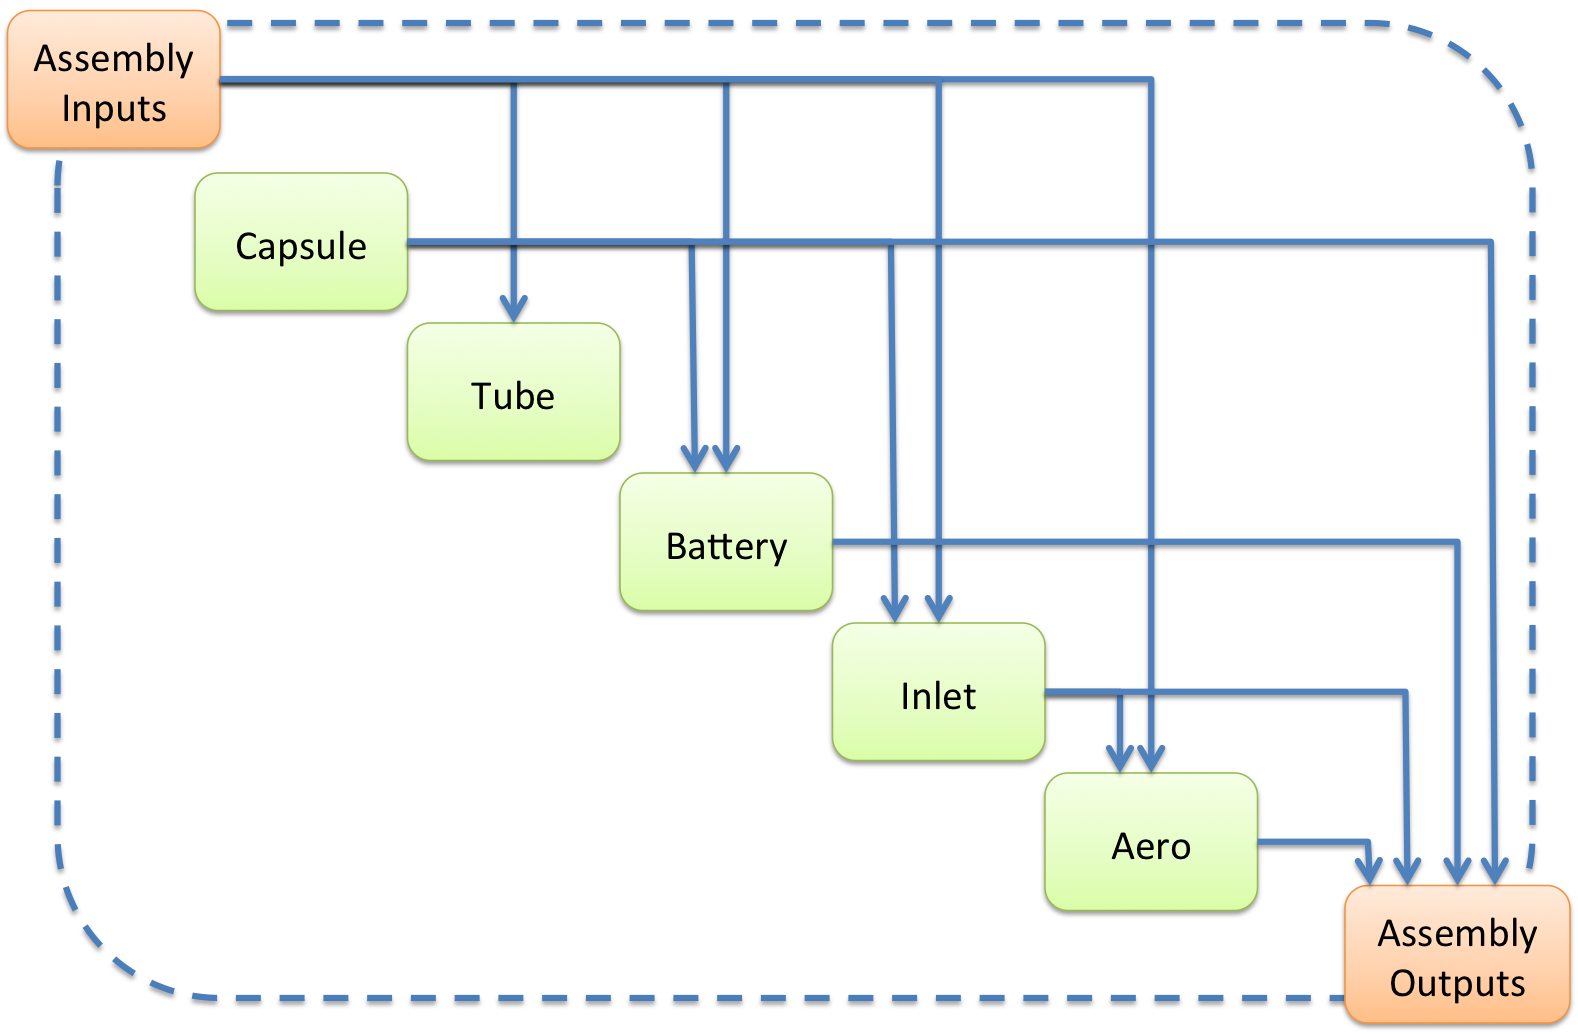
\includegraphics[width=0.65\textwidth]{images/podAssembly.png}
		\caption{Expanded pod geometry assembly}
		\label{f:podXDSM}
	\end{figure}

\section{Magnetic Levitation and Linear Induction Motors}

	\begin{figure}[hbtp]
		\centering
		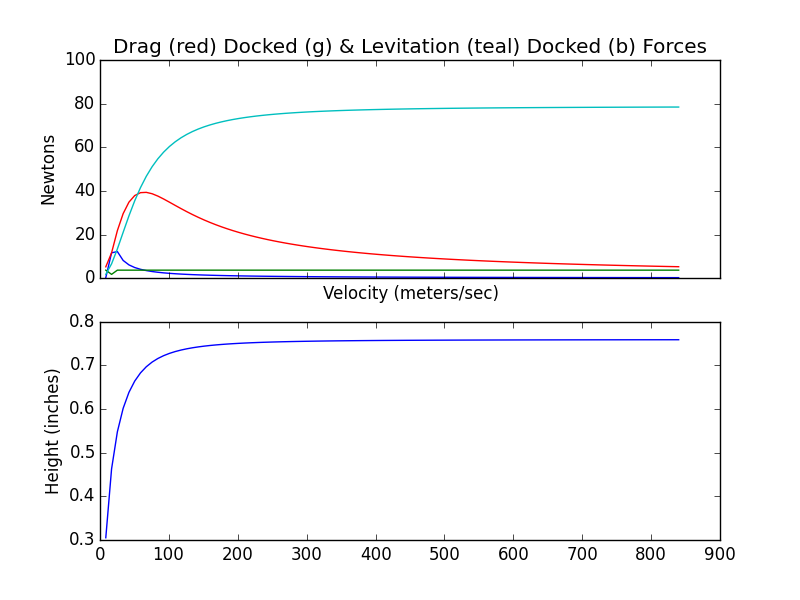
\includegraphics[width=.75\textwidth]{images/halbach0.png}
		\caption[h0]{Halbach MagLev Lift and Drag versus Vehicle Speed}
		\label{f:h0}
	\end{figure}

	\begin{figure}[hbtp]
		\centering
		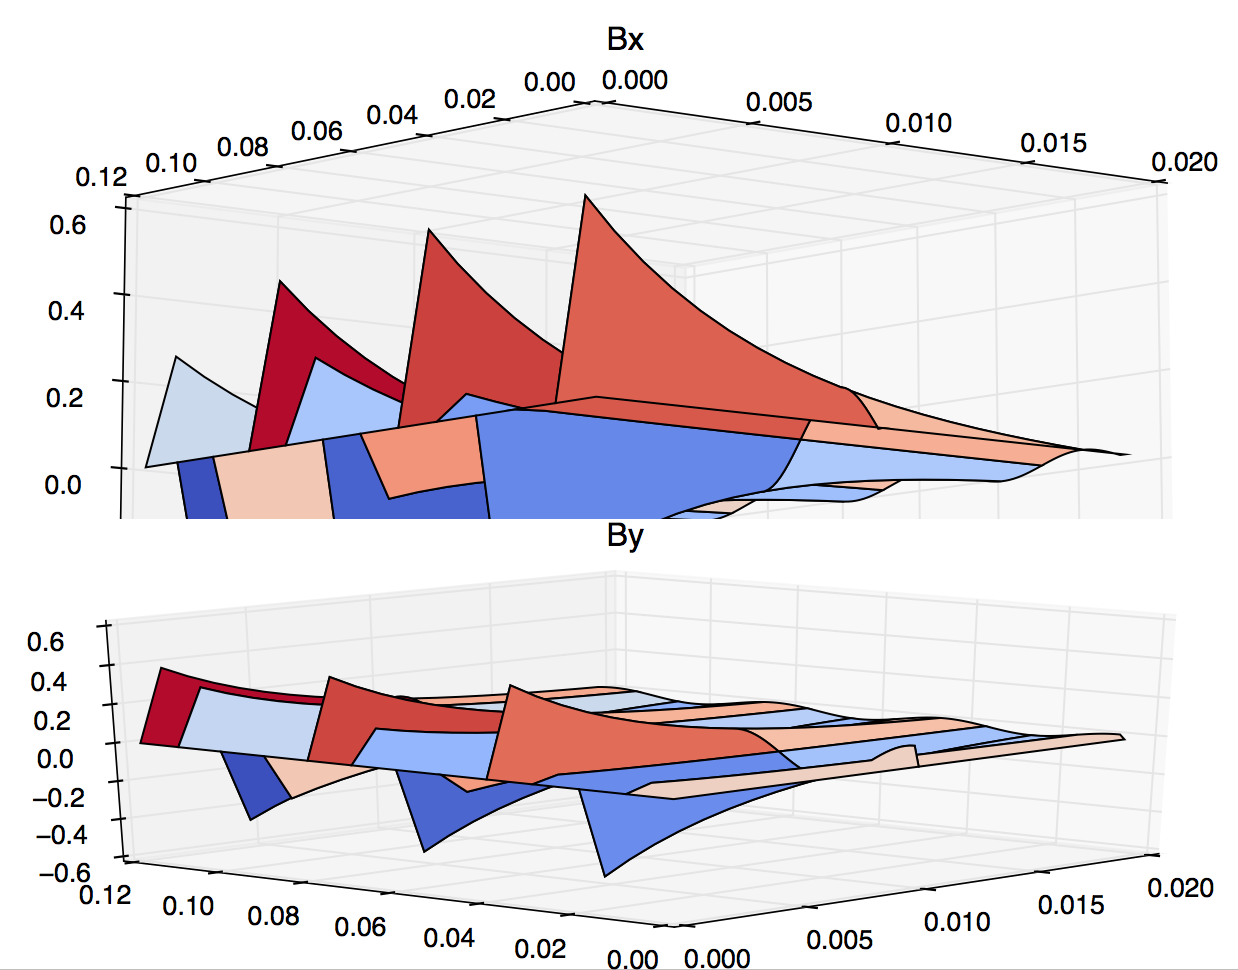
\includegraphics[width=.75\textwidth]{images/halbach1.png}
		\caption[h1]{Magnetic Flux vs distance from magnet}
		\label{f:h1}
	\end{figure}

	\begin{figure}[hbtp]
		\centering
		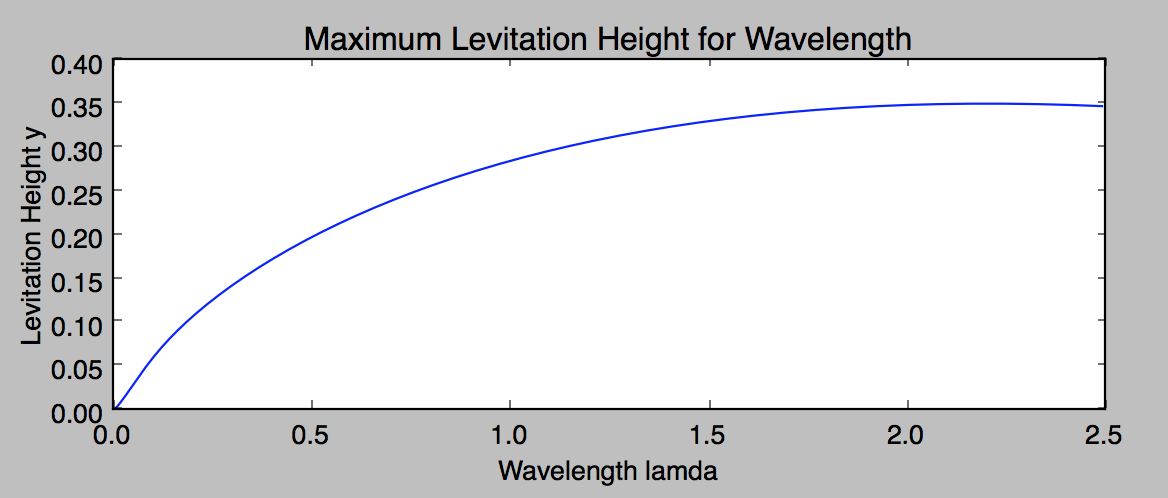
\includegraphics[width=.75\textwidth]{images/halbach2.png}
		\caption[h2]{Raw Cost per passenger vs Tube h1}
		\label{f:h2}
	\end{figure}


\section{Tube Structure and Cost}

	A trade-off exists for the distance between support pylons and tube thickness.

	\begin{figure}[hbtp]
		\centering
		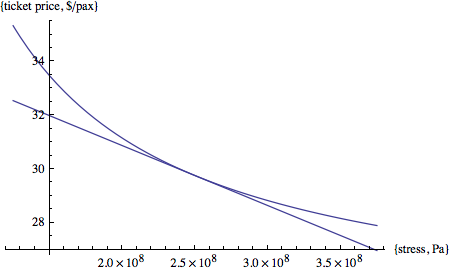
\includegraphics[width=.75\textwidth]{images/cost_stress.png}
		\caption[stress]{Raw Cost per passenger vs Tube Stress}
		\label{f:stress}
	\end{figure}

\section{Mission}

	The mission is driven by the turn radius of the vehicle at high speeds.
	To optimize the trajectory, tighter turns needed to be traded against pod speed.

\section{Aerodynamic and Compression Cycle Considerations}

	Depending on the ratio in cross-sectional area between the pod and tube,
	it may make sense to eliminate the on-board compression system.
	This would reduce the vehicle weight, but increase drag.
	The net power is tightly coupled with the rest of the system.

\section{Conclusions}

	\nomenclature{\rho}{Total, Hemispherical Reflectivity}
	\nomenclature{G}{Solar Irradiance}
	\nomenclature{c_{solar}}{Gross Irradiance Adjustment}
	\nomenclature{L}{Length (m)}
	\nomenclature{\epsilon}{Emissivity Factor}
	\nomenclature{\sigma}{Stefan-Boltzmann constant ($\frac{W}{m-K}$)}
	\nomenclature{P_{rad}}{Radiated Power (W)}
	\nomenclature{g}{Acceleration of gravity, 9.81 ($\frac{m}{s^{2}}$)}
	\nomenclature{\beta}{Volume coefficient of expansion (K)}
	\nomenclature{\upsilon}{Kinematic Viscosity ($\frac{m^{2}}{s}$)}
	\nomenclature{Pr}{Prandtl Number, $\frac{\upsilon}{\alpha}$}
	\nomenclature{Gr}{Grashof Number, $\frac{ g \beta \delta TL^{3}}{v^{2}}$}
	\nomenclature{Ra}{Rayleigh Number, $\frac{\rho U_{\infty} L}{\mu}$}
	\nomenclature{Nu}{Nusselt Number, $\frac{hL}{k}$}
	\nomenclature{h}{Heat transfer coefficient ($\frac{W}{m^{2}-K}$)}
	\nomenclature{k}{Thermal Conductivity ($\frac{W}{m-K}$) }
	\nomenclature{P}{Pressure ($\frac{N}{m^{2}}$)}
	\nomenclature{PR}{Pressure Ratio}
	\nomenclature{PR}{Pressure Ratio}
	\nomenclature{{\eta}_{ad}}{Adiabatic Efficiency}
	\nomenclature{NTU}{Number of Transfer Units}
	\nomenclature{\dot{m}}{Mass flow rate}
	\nomenclature{T}{Temperature (K)}
	\nomenclature{C_{p}}{Heat capacity at constant pressure ($\frac{J}{kg-K}$) }
	\nomenclature{Q}{Heat flow rate (W)}
	\nomenclature{\gamma}{Heat Capacity Ratio}
	\nomenclature{MN}{Mach Number}

\end{document}
